\documentclass[conference]{IEEEtran}
\usepackage[utf8]{inputenc}
\usepackage[T1]{fontenc}
\usepackage{amsmath,amssymb,amsfonts}
\usepackage{graphicx}
\usepackage{booktabs}
\usepackage{cite}
\usepackage{url}

\graphicspath{{./}{../../}}

\title{Design, Implementation, and Numerical Evaluation of the \texttt{Zvtakum} RISC-V Vector Extension for Tapered-Precision Arithmetic}

\author{
\IEEEauthorblockN{Rafael Estev\~ao, Glaucia Marques Figueiredo, and Lucas}
\IEEEauthorblockA{Departamento de Engenharia Eletr\^onica (DELT) --- Universidade Federal de Minas Gerais (UFMG)\\
Belo Horizonte, MG, Brazil\\
Email: \{rafael, glaucia, lucas\}@ufmg.br}
}

\begin{document}

\maketitle

\begin{abstract}
Low-bitwidth floating-point formats such as IEEE 754 half-precision (\texttt{FP16}) and Open Compute Project 8-bit formats (\texttt{OFP8 E4M3} and \texttt{E5M2}) are widely adopted to accelerate machine learning and scientific workloads. However, their narrow dynamic range makes them highly susceptible to numerical overflow and underflow when processing unscaled sparse matrices or wide-ranging gradients. Recently, Laslo proposed \emph{Takum}, a tapered-precision number system that guarantees a vast, bitwidth-independent dynamic range ($\approx 10^{\pm 77}$) across 8-, 16-, and 32-bit representations while concentrating precision near unity. In this paper, we present the design, implementation, and numerical evaluation of \texttt{Zvtakum}, a custom RISC-V Vector (\texttt{RVV}) instruction set extension supporting \texttt{T8}, \texttt{T16}, and \texttt{T32} formats. We design a unified 5-bit header decoder (\texttt{S, D, R}), implement core arithmetic and extended-precision dot-product instructions (\texttt{vtadd.vv}, \texttt{vtsub.vv}, \texttt{vtmul.vv}, \texttt{vtdot.vv}, and \texttt{vncvt.t.t.w}) in the \texttt{custom-1} opcode space, and evaluate them on Sparse Matrix-Vector Multiplication (SpMV) and dense General Matrix-Vector Multiplication (GEMV) workloads against a 128-bit quadruple-precision oracle (\texttt{\_\_float128}). Experimental results show that \texttt{Zvtakum} completely avoids the $100\%$ overflow/underflow failure exhibited by \texttt{OFP8} and \texttt{FP16} under wide dynamic ranges, while \texttt{vtdot.vv} reduces median relative error by $3\times$ to $7\times$ and eliminates pipeline dependencies on the \texttt{frm} and \texttt{fflags} CSRs.
\end{abstract}

\begin{IEEEkeywords}
RISC-V, Vector Extension (RVV), Takum Arithmetic, Tapered Floating-Point, SpMV, GEMV, Computer Arithmetic.
\end{IEEEkeywords}

\section{Introduction}
\label{sec:intro}

The growing computational demands of deep neural networks and large-scale scientific simulations have driven a decisive shift toward reduced-precision arithmetic. Moving from 32-bit single-precision (\texttt{FP32}) to 16-bit (\texttt{FP16}) and 8-bit (\texttt{OFP8 E4M3} and \texttt{E5M2}) representations proportionally reduces memory bandwidth bottlenecks and increases vector throughput. Nevertheless, conventional IEEE 754 floating-point formats allocate a fixed number of bits to the exponent field, creating a rigid trade-off between dynamic range and significand precision. In 8-bit formats such as \texttt{OFP8 E4M3} (maximum value $448$) and 16-bit \texttt{FP16} (maximum normal value $65504$), computations involving wide dynamic ranges frequently suffer catastrophic overflow or underflow.

To overcome these limitations, tapered-precision formats such as Posit and, more recently, \emph{Takum}~\cite{laslo2024takum} dynamically vary the length of the exponent encoding. Proposed by Laslo in 2024, Takum bounds the maximum dynamic range to roughly $e^{\pm 255} \approx 10^{\pm 77}$ regardless of the total bitwidth $N \ge 8$. Consequently, even an 8-bit Takum (\texttt{T8}) achieves a wider dynamic range than IEEE \texttt{FP32} ($\approx 10^{\pm 38}$) while retaining a shared 5-bit prefix structure (\texttt{S, D, R}) that simplifies hardware decoding across \texttt{T8}, \texttt{T16}, and \texttt{T32}.

In this work, we bridge Takum arithmetic and vector processing by proposing \texttt{Zvtakum}, a RISC-V vector extension for linear Takum arithmetic. The main contributions of this work are:
\begin{itemize}
    \item A unified hardware-oriented C++ core and decoder for \texttt{T8}, \texttt{T16}, and \texttt{T32} validated against \texttt{libtakum} and numerical quadrature rules;
    \item The specification and functional simulation of the \texttt{Zvtakum} ISA extension within the RISC-V \texttt{custom-1} opcode space, including an extended-precision vector dot product (\texttt{vtdot.vv});
    \item A comprehensive numerical and architectural evaluation across CSR SpMV and dense ML GEMV workloads against an IEEE 754 quadruple-precision (\texttt{\_\_float128}) oracle, alongside an instruction count and CSR overhead analysis.
\end{itemize}

\section{Background and Related Work}
\label{sec:background}

\subsection{IEEE 754, OCP FP8, and Tapered-Precision Arithmetic}
In IEEE 754 floating-point representations, a real number is encoded using a sign bit $S$, a fixed-width biased exponent $E$, and a significand fraction $M$. Shrinking the word size to 16 or 8 bits severely restricts the exponent field. The Open Compute Project (OCP) defines two 8-bit variants~\cite{ocp_fp8}: \texttt{E4M3} (saturating at $\pm 448$) and \texttt{E5M2} (range $\pm 57344$). Both formats exhibit high quantization noise and rapid saturation when matrix entries span multiple orders of magnitude. Posit arithmetic~\cite{gustafson2017posit} introduced a variable-length unary regime field to provide higher precision near $1.0$, but its variable-length regime requires a full-word leading-zero/one detector before exponent extraction.

\subsection{The Linear Takum Format}
Takum arithmetic~\cite{laslo2024takum} replaces the unbounded unary regime with a fixed 3-bit regime field $R$ combined with a direction bit $D$ and sign bit $S$. For an $n$-bit Takum (\texttt{T8}, \texttt{T16}, or \texttt{T32}), the first 5 bits $(S, D, R)$ completely determine the bitwidth $r$ of the characteristic field $C$:
\begin{equation}
    r = \begin{cases} R, & \text{if } D = 1 \\ 7 - R, & \text{if } D = 0 \end{cases}
\end{equation}
The signed characteristic $c$ and the remaining $p = n - 5 - r$ mantissa bits $M$ yield a linear floating-point value $(-1)^S \cdot 2^c \cdot (1 + M / 2^p)$. Because only the first 5 bits must be inspected to locate $C$ and $M$, the decoder front-end is identical across \texttt{T8}, \texttt{T16}, and \texttt{T32}.

\subsection{RISC-V Vector Extension (RVV)}
The RISC-V Vector Extension (\texttt{RVV 1.0})~\cite{riscv_v_spec} employs a vector-length agnostic programming model governed by \texttt{vtype} (which configures \texttt{SEW} and \texttt{LMUL}) and \texttt{vl} (active vector length). Application loops use \texttt{vsetvli} to strip-mine arbitrary-length vectors across different hardware vector register widths (\texttt{VLEN}).

% Seção "Proposed Architecture" (Rafael). Incluir no artigo com % Seção "Proposed Architecture" (Rafael). Incluir no artigo com % Seção "Proposed Architecture" (Rafael). Incluir no artigo com \input{secao_arquitetura}.
% Requer: \usepackage{graphicx,booktabs,amsmath,tikz}  (template IEEEtran)
\section{Proposed Architecture}
\label{sec:arch}

We implemented the Takum datapath as a bit-exact C++ functional model and integrated
it into the Spike RISC-V ISA simulator as the \emph{Zvtakum} vector extension. The
simulator was chosen over an RTL description because it allowed us to validate
millions of operations against a reference library and to reuse the \emph{same} source
file inside the ISA simulator, so no second copy of the arithmetic exists.

\subsection{Format and Decoder}
We use the linear takum of Hunhold~\cite{hunhold2024takum} with $n\in\{8,16,32\}$ bits:
\begin{equation}
\underbrace{S}_{1}\,\underbrace{D}_{1}\,\underbrace{R}_{3}\,\underbrace{C}_{r}\,\underbrace{M}_{p},
\qquad r = D\,?\,R : 7-R,\quad p = n-5-r .
\end{equation}
The regime field has a fixed width of three bits, so the number of characteristic
bits $r$ is known after reading only the first five bits ($S$, $D$, $R$). This is the
property that gives takums a decoder whose front end is common to all widths~\cite{hunhold2025avx}.
The characteristic is $c = 2^r-1+C$ for $D=1$ and $c=-2^{r+1}+1+C$ for $D=0$, and the
mantissa is $1.f$ with $f=M/2^p$. In T8 the characteristic may not fit in the
remaining bits; it is then truncated and completed with zeros. The all-zero pattern is the
only zero and $10\ldots0$ is the only NaR (not-a-real); there are no infinities and no NaN payloads.

The decoder is organised in two layers: (i)~field extraction (S, D, R, C, M and the derived $r$, $c$, $p$),
and (ii)~an internal triple (sign, exponent, 64-bit significand) on which the ALU operates.

\subsection{Arithmetic Unit}
Addition, subtraction, multiplication and division share a single encoder. The product of two
significands is computed exactly in 128 bits; the adder aligns exponents in 128 bits with
62 guard bits plus a sticky bit, and subtraction renormalises by the leading one after cancellation.
Results are rounded to nearest, ties to even, on the bit string $(D\,R\,C\,M)$, which
is what the reference library does, and they saturate: overflow never produces NaR and
underflow never produces zero. NaR propagates through every operation.
Because every operation acts on bit patterns, width conversion (\texttt{vncvt.t.t}) reduces to the
encoder's rounding step. Rounding has a single mode and there are no exception flags;
this is the basis of the CSR analysis in Section~\ref{sec:results}.

\subsection{The Zvtakum Extension}
Zvtakum adds five instructions (Table~\ref{tab:zvt}) that operate on elements whose width equals
\texttt{SEW}, reusing \texttt{vl}, \texttt{vstart}, the mask bit and register grouping of
the standard vector extension. SEW$=64$ is illegal because the project has no T64.
The instructions are placed in the \emph{custom-1} opcode space (\texttt{0x2b}) with the OP-V field layout, because the
reserved OP-V slots belong to RISC-V International.

\begin{table}[t]
\caption{Zvtakum instructions (opcode \texttt{0x2b}, \texttt{funct3}$=000$).}
\label{tab:zvt}
\centering
\small
\begin{tabular}{@{}lll@{}}
\toprule
Instruction & \texttt{funct6} & Semantics \\
\midrule
\texttt{vtadd.vv}  & 000000 & $vd_i = vs2_i + vs1_i$ \\
\texttt{vtsub.vv}  & 000001 & $vd_i = vs2_i - vs1_i$ \\
\texttt{vtmul.vv}  & 000010 & $vd_i = vs2_i \cdot vs1_i$ \\
\texttt{vtdot.vv}  & 000011 & $vd_0 = \mathrm{RN}(vd_0+\sum_i vs2_i\,vs1_i)$ \\
\texttt{vncvt.t.t} & 000100 & $vd_i=\mathrm{RN}_{SEW}(vs2_i)$, $vs2$ is $2\!\cdot\!$SEW \\
\bottomrule
\end{tabular}
\end{table}

\textbf{Operand order.} \texttt{vtsub} computes $vs2-vs1$, like \texttt{vfsub.vv}.

\textbf{Dot product.} \texttt{vtdot.vv} is a reduction: \texttt{vd} is an accumulator (as in \texttt{vmacc}), only
element~0 is read and written, and the instruction requires \texttt{vstart}$=0$. Each product is exact (at most 56
significand bits) and is added to an accumulator with a 64-bit significand, more than twice the 27 fraction bits of T32;
only one rounding to SEW bits happens at the end. We considered two alternatives. A widened destination
(T8$\rightarrow$T16, T16$\rightarrow$T32) is not uniform because T32 would need a T64. An exact accumulator (quire, about
1.2\,kbit) is more faithful but far more expensive in hardware. Our choice is uniform across widths; its cost is that a cancellation of more
than $\approx$64 bits loses the residual, which only happens with extreme dynamic range (random T8 bit patterns).
In strip-mined loops each \texttt{vtdot} stores a partial result rounded to SEW bits, and our experiments model exactly this behaviour.

\subsection{Simulator Integration and Validation}
In Spike, the five instructions are implemented as \texttt{insns/*.h} files that call the project's decoder
through a thin glue unit. They are registered in \texttt{encoding.h}, in the build list and in the
disassembler, so traces show them by name. Validation has three layers:
(i)~decode/encode and $+,-,\times,\div$ against \texttt{libtakum}, exhaustively in T8 and with $12$~M random operations each in T16 and T32 (0 mismatches);
(ii)~\texttt{takum\_dot} against \texttt{\_\_float128} and, bit by bit, against an independent Python model with exact rationals (11{,}643 cases, 0 mismatches);
(iii)~a bare-metal program run in Spike with \texttt{--isa=rv64gv} that executes the five instructions with full and partial \texttt{vl}, masks, NaR, zero,
SEW$=8/16/32$ and register groups, and compares with the expected values (22 instruction tests pass; a negative control with corrupted
expected values fails as it should).
.
% Requer: \usepackage{graphicx,booktabs,amsmath,tikz}  (template IEEEtran)
\section{Proposed Architecture}
\label{sec:arch}

We implemented the Takum datapath as a bit-exact C++ functional model and integrated
it into the Spike RISC-V ISA simulator as the \emph{Zvtakum} vector extension. The
simulator was chosen over an RTL description because it allowed us to validate
millions of operations against a reference library and to reuse the \emph{same} source
file inside the ISA simulator, so no second copy of the arithmetic exists.

\subsection{Format and Decoder}
We use the linear takum of Hunhold~\cite{hunhold2024takum} with $n\in\{8,16,32\}$ bits:
\begin{equation}
\underbrace{S}_{1}\,\underbrace{D}_{1}\,\underbrace{R}_{3}\,\underbrace{C}_{r}\,\underbrace{M}_{p},
\qquad r = D\,?\,R : 7-R,\quad p = n-5-r .
\end{equation}
The regime field has a fixed width of three bits, so the number of characteristic
bits $r$ is known after reading only the first five bits ($S$, $D$, $R$). This is the
property that gives takums a decoder whose front end is common to all widths~\cite{hunhold2025avx}.
The characteristic is $c = 2^r-1+C$ for $D=1$ and $c=-2^{r+1}+1+C$ for $D=0$, and the
mantissa is $1.f$ with $f=M/2^p$. In T8 the characteristic may not fit in the
remaining bits; it is then truncated and completed with zeros. The all-zero pattern is the
only zero and $10\ldots0$ is the only NaR (not-a-real); there are no infinities and no NaN payloads.

The decoder is organised in two layers: (i)~field extraction (S, D, R, C, M and the derived $r$, $c$, $p$),
and (ii)~an internal triple (sign, exponent, 64-bit significand) on which the ALU operates.

\subsection{Arithmetic Unit}
Addition, subtraction, multiplication and division share a single encoder. The product of two
significands is computed exactly in 128 bits; the adder aligns exponents in 128 bits with
62 guard bits plus a sticky bit, and subtraction renormalises by the leading one after cancellation.
Results are rounded to nearest, ties to even, on the bit string $(D\,R\,C\,M)$, which
is what the reference library does, and they saturate: overflow never produces NaR and
underflow never produces zero. NaR propagates through every operation.
Because every operation acts on bit patterns, width conversion (\texttt{vncvt.t.t}) reduces to the
encoder's rounding step. Rounding has a single mode and there are no exception flags;
this is the basis of the CSR analysis in Section~\ref{sec:results}.

\subsection{The Zvtakum Extension}
Zvtakum adds five instructions (Table~\ref{tab:zvt}) that operate on elements whose width equals
\texttt{SEW}, reusing \texttt{vl}, \texttt{vstart}, the mask bit and register grouping of
the standard vector extension. SEW$=64$ is illegal because the project has no T64.
The instructions are placed in the \emph{custom-1} opcode space (\texttt{0x2b}) with the OP-V field layout, because the
reserved OP-V slots belong to RISC-V International.

\begin{table}[t]
\caption{Zvtakum instructions (opcode \texttt{0x2b}, \texttt{funct3}$=000$).}
\label{tab:zvt}
\centering
\small
\begin{tabular}{@{}lll@{}}
\toprule
Instruction & \texttt{funct6} & Semantics \\
\midrule
\texttt{vtadd.vv}  & 000000 & $vd_i = vs2_i + vs1_i$ \\
\texttt{vtsub.vv}  & 000001 & $vd_i = vs2_i - vs1_i$ \\
\texttt{vtmul.vv}  & 000010 & $vd_i = vs2_i \cdot vs1_i$ \\
\texttt{vtdot.vv}  & 000011 & $vd_0 = \mathrm{RN}(vd_0+\sum_i vs2_i\,vs1_i)$ \\
\texttt{vncvt.t.t} & 000100 & $vd_i=\mathrm{RN}_{SEW}(vs2_i)$, $vs2$ is $2\!\cdot\!$SEW \\
\bottomrule
\end{tabular}
\end{table}

\textbf{Operand order.} \texttt{vtsub} computes $vs2-vs1$, like \texttt{vfsub.vv}.

\textbf{Dot product.} \texttt{vtdot.vv} is a reduction: \texttt{vd} is an accumulator (as in \texttt{vmacc}), only
element~0 is read and written, and the instruction requires \texttt{vstart}$=0$. Each product is exact (at most 56
significand bits) and is added to an accumulator with a 64-bit significand, more than twice the 27 fraction bits of T32;
only one rounding to SEW bits happens at the end. We considered two alternatives. A widened destination
(T8$\rightarrow$T16, T16$\rightarrow$T32) is not uniform because T32 would need a T64. An exact accumulator (quire, about
1.2\,kbit) is more faithful but far more expensive in hardware. Our choice is uniform across widths; its cost is that a cancellation of more
than $\approx$64 bits loses the residual, which only happens with extreme dynamic range (random T8 bit patterns).
In strip-mined loops each \texttt{vtdot} stores a partial result rounded to SEW bits, and our experiments model exactly this behaviour.

\subsection{Simulator Integration and Validation}
In Spike, the five instructions are implemented as \texttt{insns/*.h} files that call the project's decoder
through a thin glue unit. They are registered in \texttt{encoding.h}, in the build list and in the
disassembler, so traces show them by name. Validation has three layers:
(i)~decode/encode and $+,-,\times,\div$ against \texttt{libtakum}, exhaustively in T8 and with $12$~M random operations each in T16 and T32 (0 mismatches);
(ii)~\texttt{takum\_dot} against \texttt{\_\_float128} and, bit by bit, against an independent Python model with exact rationals (11{,}643 cases, 0 mismatches);
(iii)~a bare-metal program run in Spike with \texttt{--isa=rv64gv} that executes the five instructions with full and partial \texttt{vl}, masks, NaR, zero,
SEW$=8/16/32$ and register groups, and compares with the expected values (22 instruction tests pass; a negative control with corrupted
expected values fails as it should).
.
% Requer: \usepackage{graphicx,booktabs,amsmath,tikz}  (template IEEEtran)
\section{Proposed Architecture}
\label{sec:arch}

We implemented the Takum datapath as a bit-exact C++ functional model and integrated
it into the Spike RISC-V ISA simulator as the \emph{Zvtakum} vector extension. The
simulator was chosen over an RTL description because it allowed us to validate
millions of operations against a reference library and to reuse the \emph{same} source
file inside the ISA simulator, so no second copy of the arithmetic exists.

\subsection{Format and Decoder}
We use the linear takum of Hunhold~\cite{hunhold2024takum} with $n\in\{8,16,32\}$ bits:
\begin{equation}
\underbrace{S}_{1}\,\underbrace{D}_{1}\,\underbrace{R}_{3}\,\underbrace{C}_{r}\,\underbrace{M}_{p},
\qquad r = D\,?\,R : 7-R,\quad p = n-5-r .
\end{equation}
The regime field has a fixed width of three bits, so the number of characteristic
bits $r$ is known after reading only the first five bits ($S$, $D$, $R$). This is the
property that gives takums a decoder whose front end is common to all widths~\cite{hunhold2025avx}.
The characteristic is $c = 2^r-1+C$ for $D=1$ and $c=-2^{r+1}+1+C$ for $D=0$, and the
mantissa is $1.f$ with $f=M/2^p$. In T8 the characteristic may not fit in the
remaining bits; it is then truncated and completed with zeros. The all-zero pattern is the
only zero and $10\ldots0$ is the only NaR (not-a-real); there are no infinities and no NaN payloads.

The decoder is organised in two layers: (i)~field extraction (S, D, R, C, M and the derived $r$, $c$, $p$),
and (ii)~an internal triple (sign, exponent, 64-bit significand) on which the ALU operates.

\subsection{Arithmetic Unit}
Addition, subtraction, multiplication and division share a single encoder. The product of two
significands is computed exactly in 128 bits; the adder aligns exponents in 128 bits with
62 guard bits plus a sticky bit, and subtraction renormalises by the leading one after cancellation.
Results are rounded to nearest, ties to even, on the bit string $(D\,R\,C\,M)$, which
is what the reference library does, and they saturate: overflow never produces NaR and
underflow never produces zero. NaR propagates through every operation.
Because every operation acts on bit patterns, width conversion (\texttt{vncvt.t.t}) reduces to the
encoder's rounding step. Rounding has a single mode and there are no exception flags;
this is the basis of the CSR analysis in Section~\ref{sec:results}.

\subsection{The Zvtakum Extension}
Zvtakum adds five instructions (Table~\ref{tab:zvt}) that operate on elements whose width equals
\texttt{SEW}, reusing \texttt{vl}, \texttt{vstart}, the mask bit and register grouping of
the standard vector extension. SEW$=64$ is illegal because the project has no T64.
The instructions are placed in the \emph{custom-1} opcode space (\texttt{0x2b}) with the OP-V field layout, because the
reserved OP-V slots belong to RISC-V International.

\begin{table}[t]
\caption{Zvtakum instructions (opcode \texttt{0x2b}, \texttt{funct3}$=000$).}
\label{tab:zvt}
\centering
\small
\begin{tabular}{@{}lll@{}}
\toprule
Instruction & \texttt{funct6} & Semantics \\
\midrule
\texttt{vtadd.vv}  & 000000 & $vd_i = vs2_i + vs1_i$ \\
\texttt{vtsub.vv}  & 000001 & $vd_i = vs2_i - vs1_i$ \\
\texttt{vtmul.vv}  & 000010 & $vd_i = vs2_i \cdot vs1_i$ \\
\texttt{vtdot.vv}  & 000011 & $vd_0 = \mathrm{RN}(vd_0+\sum_i vs2_i\,vs1_i)$ \\
\texttt{vncvt.t.t} & 000100 & $vd_i=\mathrm{RN}_{SEW}(vs2_i)$, $vs2$ is $2\!\cdot\!$SEW \\
\bottomrule
\end{tabular}
\end{table}

\textbf{Operand order.} \texttt{vtsub} computes $vs2-vs1$, like \texttt{vfsub.vv}.

\textbf{Dot product.} \texttt{vtdot.vv} is a reduction: \texttt{vd} is an accumulator (as in \texttt{vmacc}), only
element~0 is read and written, and the instruction requires \texttt{vstart}$=0$. Each product is exact (at most 56
significand bits) and is added to an accumulator with a 64-bit significand, more than twice the 27 fraction bits of T32;
only one rounding to SEW bits happens at the end. We considered two alternatives. A widened destination
(T8$\rightarrow$T16, T16$\rightarrow$T32) is not uniform because T32 would need a T64. An exact accumulator (quire, about
1.2\,kbit) is more faithful but far more expensive in hardware. Our choice is uniform across widths; its cost is that a cancellation of more
than $\approx$64 bits loses the residual, which only happens with extreme dynamic range (random T8 bit patterns).
In strip-mined loops each \texttt{vtdot} stores a partial result rounded to SEW bits, and our experiments model exactly this behaviour.

\subsection{Simulator Integration and Validation}
In Spike, the five instructions are implemented as \texttt{insns/*.h} files that call the project's decoder
through a thin glue unit. They are registered in \texttt{encoding.h}, in the build list and in the
disassembler, so traces show them by name. Validation has three layers:
(i)~decode/encode and $+,-,\times,\div$ against \texttt{libtakum}, exhaustively in T8 and with $12$~M random operations each in T16 and T32 (0 mismatches);
(ii)~\texttt{takum\_dot} against \texttt{\_\_float128} and, bit by bit, against an independent Python model with exact rationals (11{,}643 cases, 0 mismatches);
(iii)~a bare-metal program run in Spike with \texttt{--isa=rv64gv} that executes the five instructions with full and partial \texttt{vl}, masks, NaR, zero,
SEW$=8/16/32$ and register groups, and compares with the expected values (22 instruction tests pass; a negative control with corrupted
expected values fails as it should).

\section{Results and Discussion}
\label{sec:results}

\subsection{Experimental Setup and Quadruple-Precision Oracle}
To evaluate the numerical behavior of the proposed \texttt{Zvtakum} extension across scientific computing and machine learning workloads, we evaluate three benchmarks: (i) composite numerical quadrature rules (\texttt{make integracao}), (ii) Sparse Matrix-Vector Multiplication (SpMV) in Compressed Sparse Row (CSR) format, and (iii) a dense General Matrix-Vector Multiplication (GEMV) kernel. Unlike standard x86-64 \texttt{long double} (80-bit extended format with a 64-bit significand), our ground-truth reference $y_{\text{ref}}$ is computed in IEEE 754 quadruple precision (\texttt{\_\_float128} via \texttt{libquadmath}, providing 113 significand bits).

We compare linear Takum (\texttt{T8}, \texttt{T16}, \texttt{T32}) against IEEE 754~\cite{ieee754} \texttt{FP32} and \texttt{FP16}, as well as Open Compute Project (OCP) 8-bit formats~\cite{ocp_fp8} \texttt{OFP8 E4M3} (normal range up to $\pm 448$) and \texttt{OFP8 E5M2} (range up to $\pm 57344$). Two matrix dimensions are evaluated: $200 \times 200$ ($d = 10\%$, averaging 20 non-zeros per row) to exercise non-power-of-two strip-mining tails ($\texttt{vl} < \texttt{VLEN}/\texttt{SEW}$), and power-of-two dimensions ($256 \times 256$ SpMV with $d = 10\%, 20\%$ and $128 \times 128$ dense GEMV) that align evenly with a 128-bit vector register width ($\texttt{VLEN} = 128$, yielding $\texttt{vl} \in \{16, 8, 4\}$ elements per strip for \texttt{T8}, \texttt{T16}, and \texttt{T32}). To avoid division-by-near-zero distortion in element-wise relative error $\vert{}y_i - y_{\text{ref},i}\vert{} / \vert{}y_{\text{ref},i}\vert{}$, reference outputs satisfying $\vert{}y_{\text{ref},i}\vert{} \le 10^{-12} \max_j \vert{}y_{\text{ref},j}\vert{}$ are filtered out across 15 random seeds.

\subsection{Numerical Quadrature Validation}
Prior to vector workload evaluation, the arithmetic core was validated on composite numerical integration (trapezoidal quadrature of smooth transcendental integrands) across increasing subinterval counts $N$. Figure~\ref{fig:quadrature} illustrates the relative integration error as a function of discretization granularity. Both \texttt{T16} and \texttt{T32} closely track or surpass their IEEE counterparts before reaching rounding saturation, while \texttt{T8} remains bounded without catastrophic overflow as $N$ grows.

\begin{figure}[htbp]
\centering
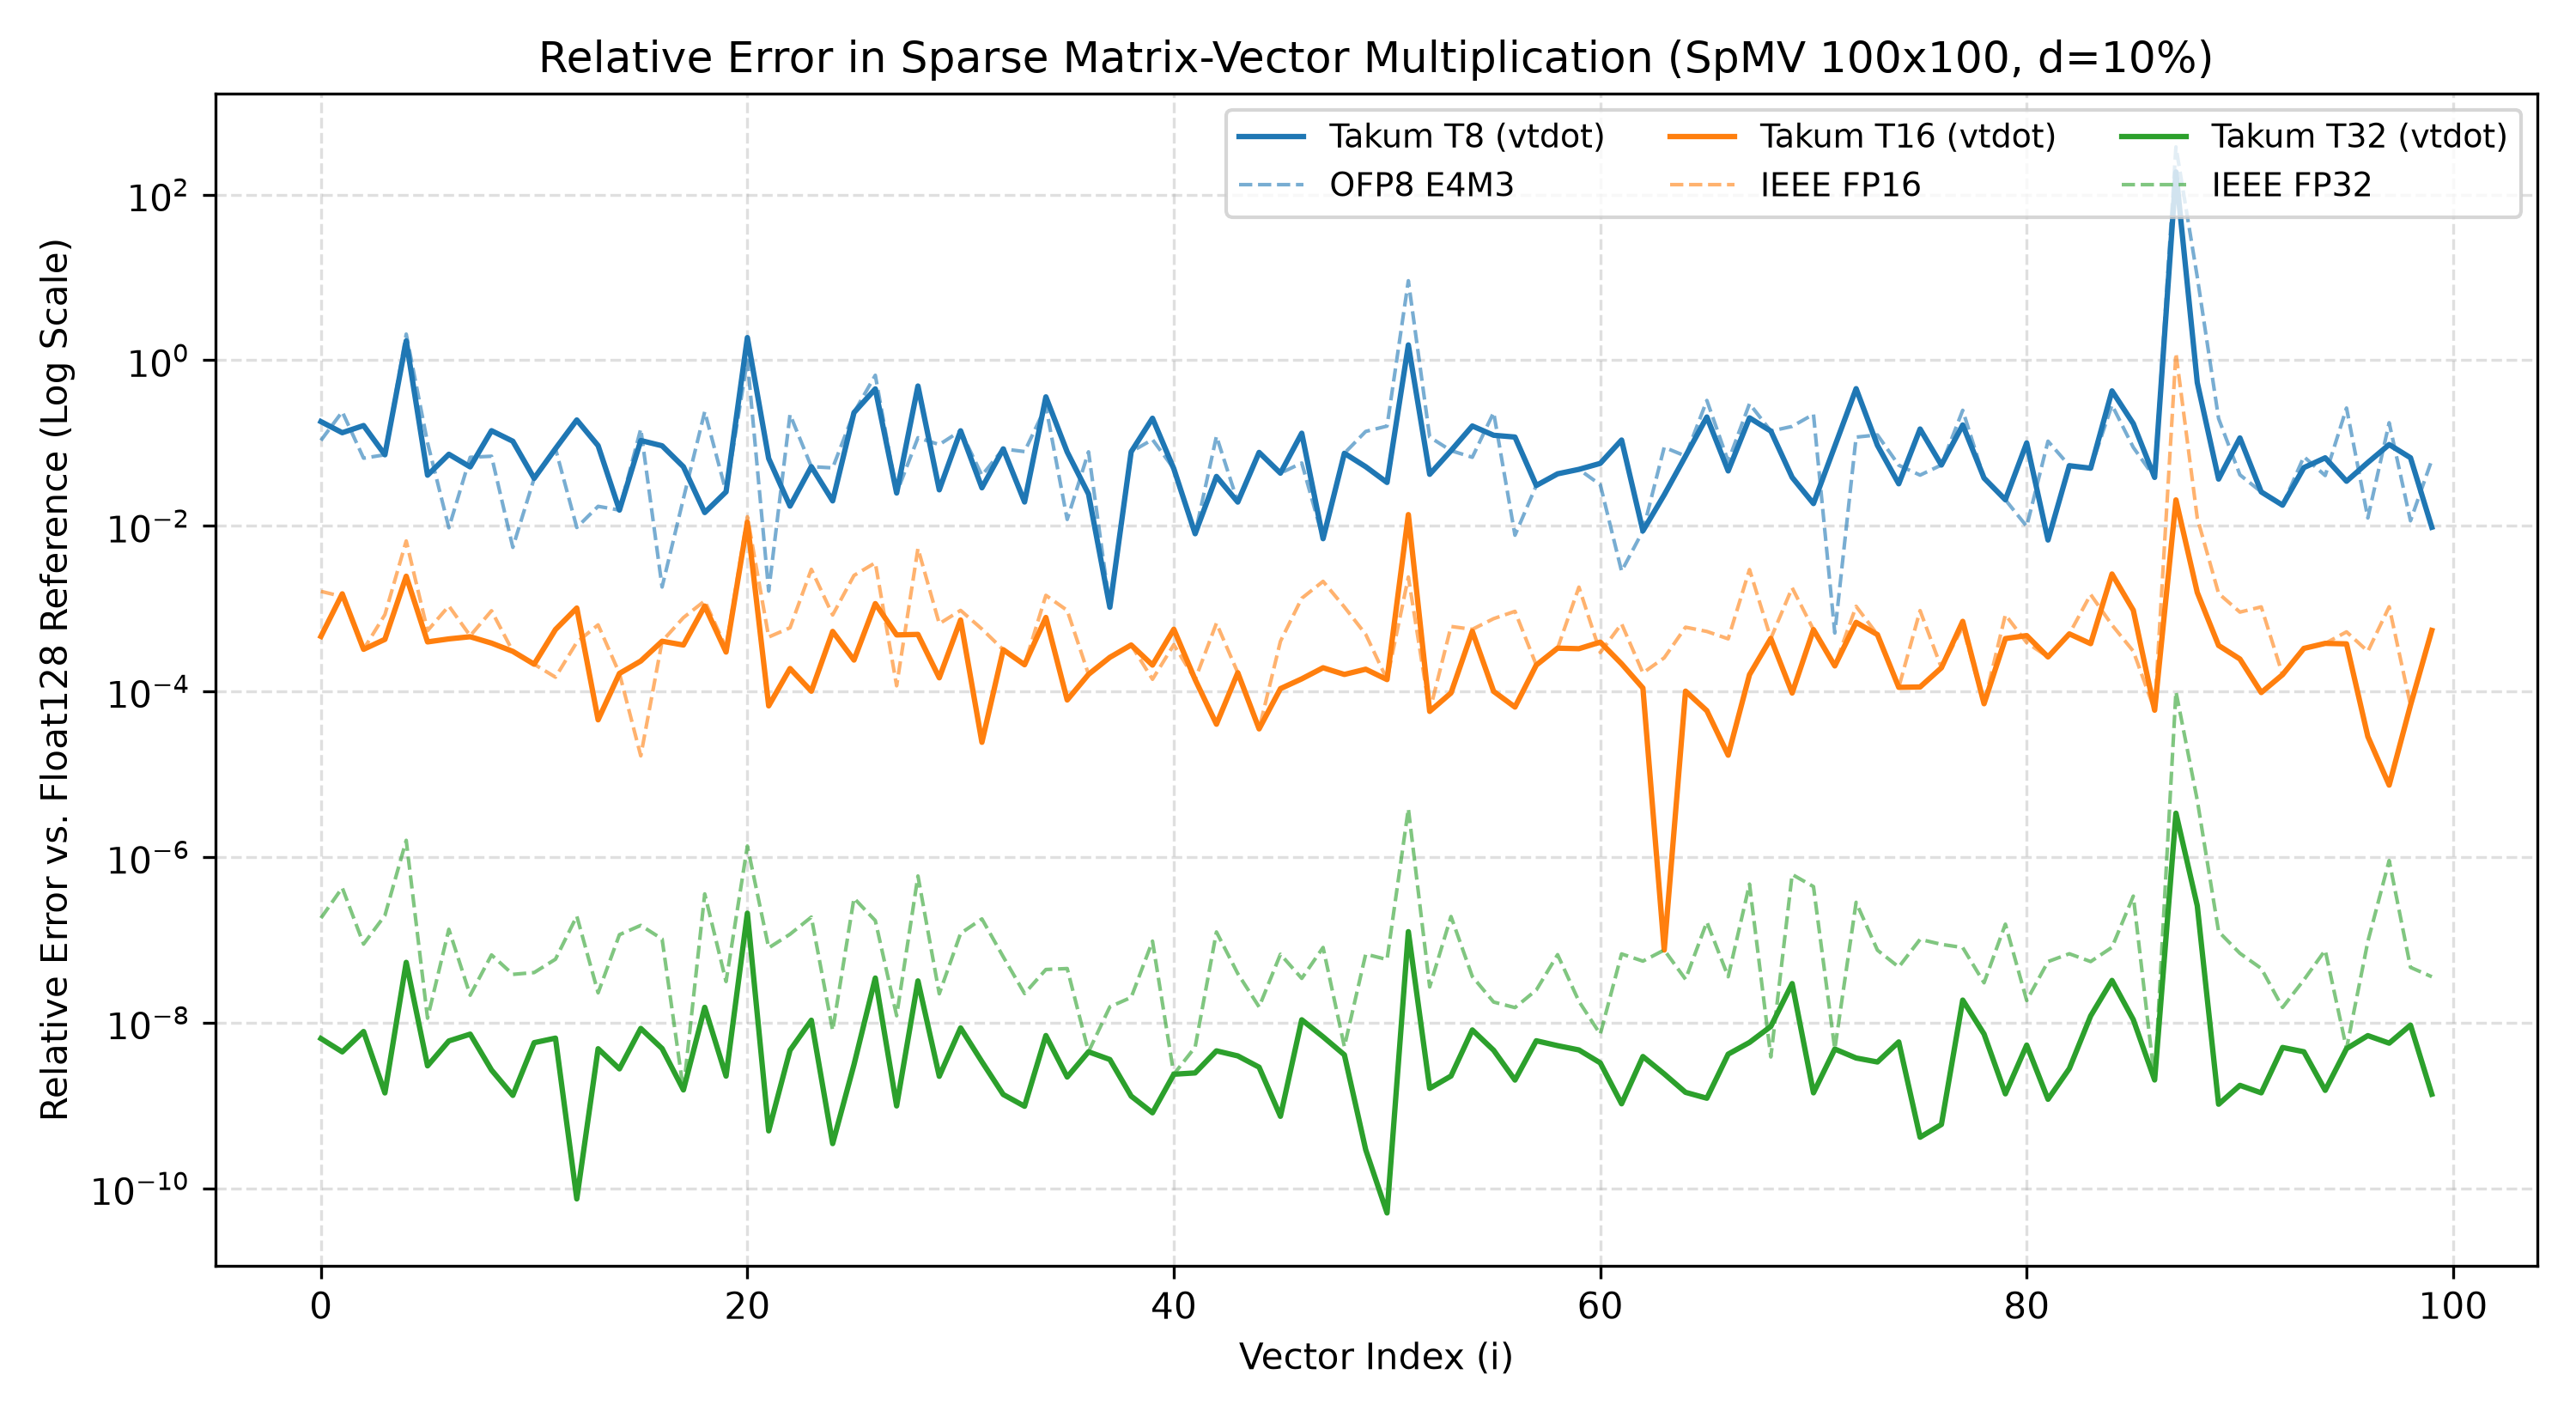
\includegraphics[width=0.95\columnwidth]{grafico_erro_takum.png}
\caption{Relative error in numerical quadrature validation across bitwidths.}
\label{fig:quadrature}
\end{figure}

\subsection{SpMV Accuracy: Narrow vs. Wide Dynamic Range}
Figure~\ref{fig:spmv_cdf} presents the Cumulative Distribution Function (CDF) of the element-wise relative error for $200 \times 200$ CSR sparse matrices ($d = 10\%$) under two input distributions: (a) a narrow standard normal regime $\mathcal{N}(0, 1)$, and (b) a wide dynamic range regime $\mathcal{N}(0, 1) \cdot 2^{\mathcal{U}(-18, 18)}$ whose products span roughly $2^{-36}$ to $2^{+36}$ ($\approx 10^{\pm 11}$).

\begin{figure*}[t]
\centering
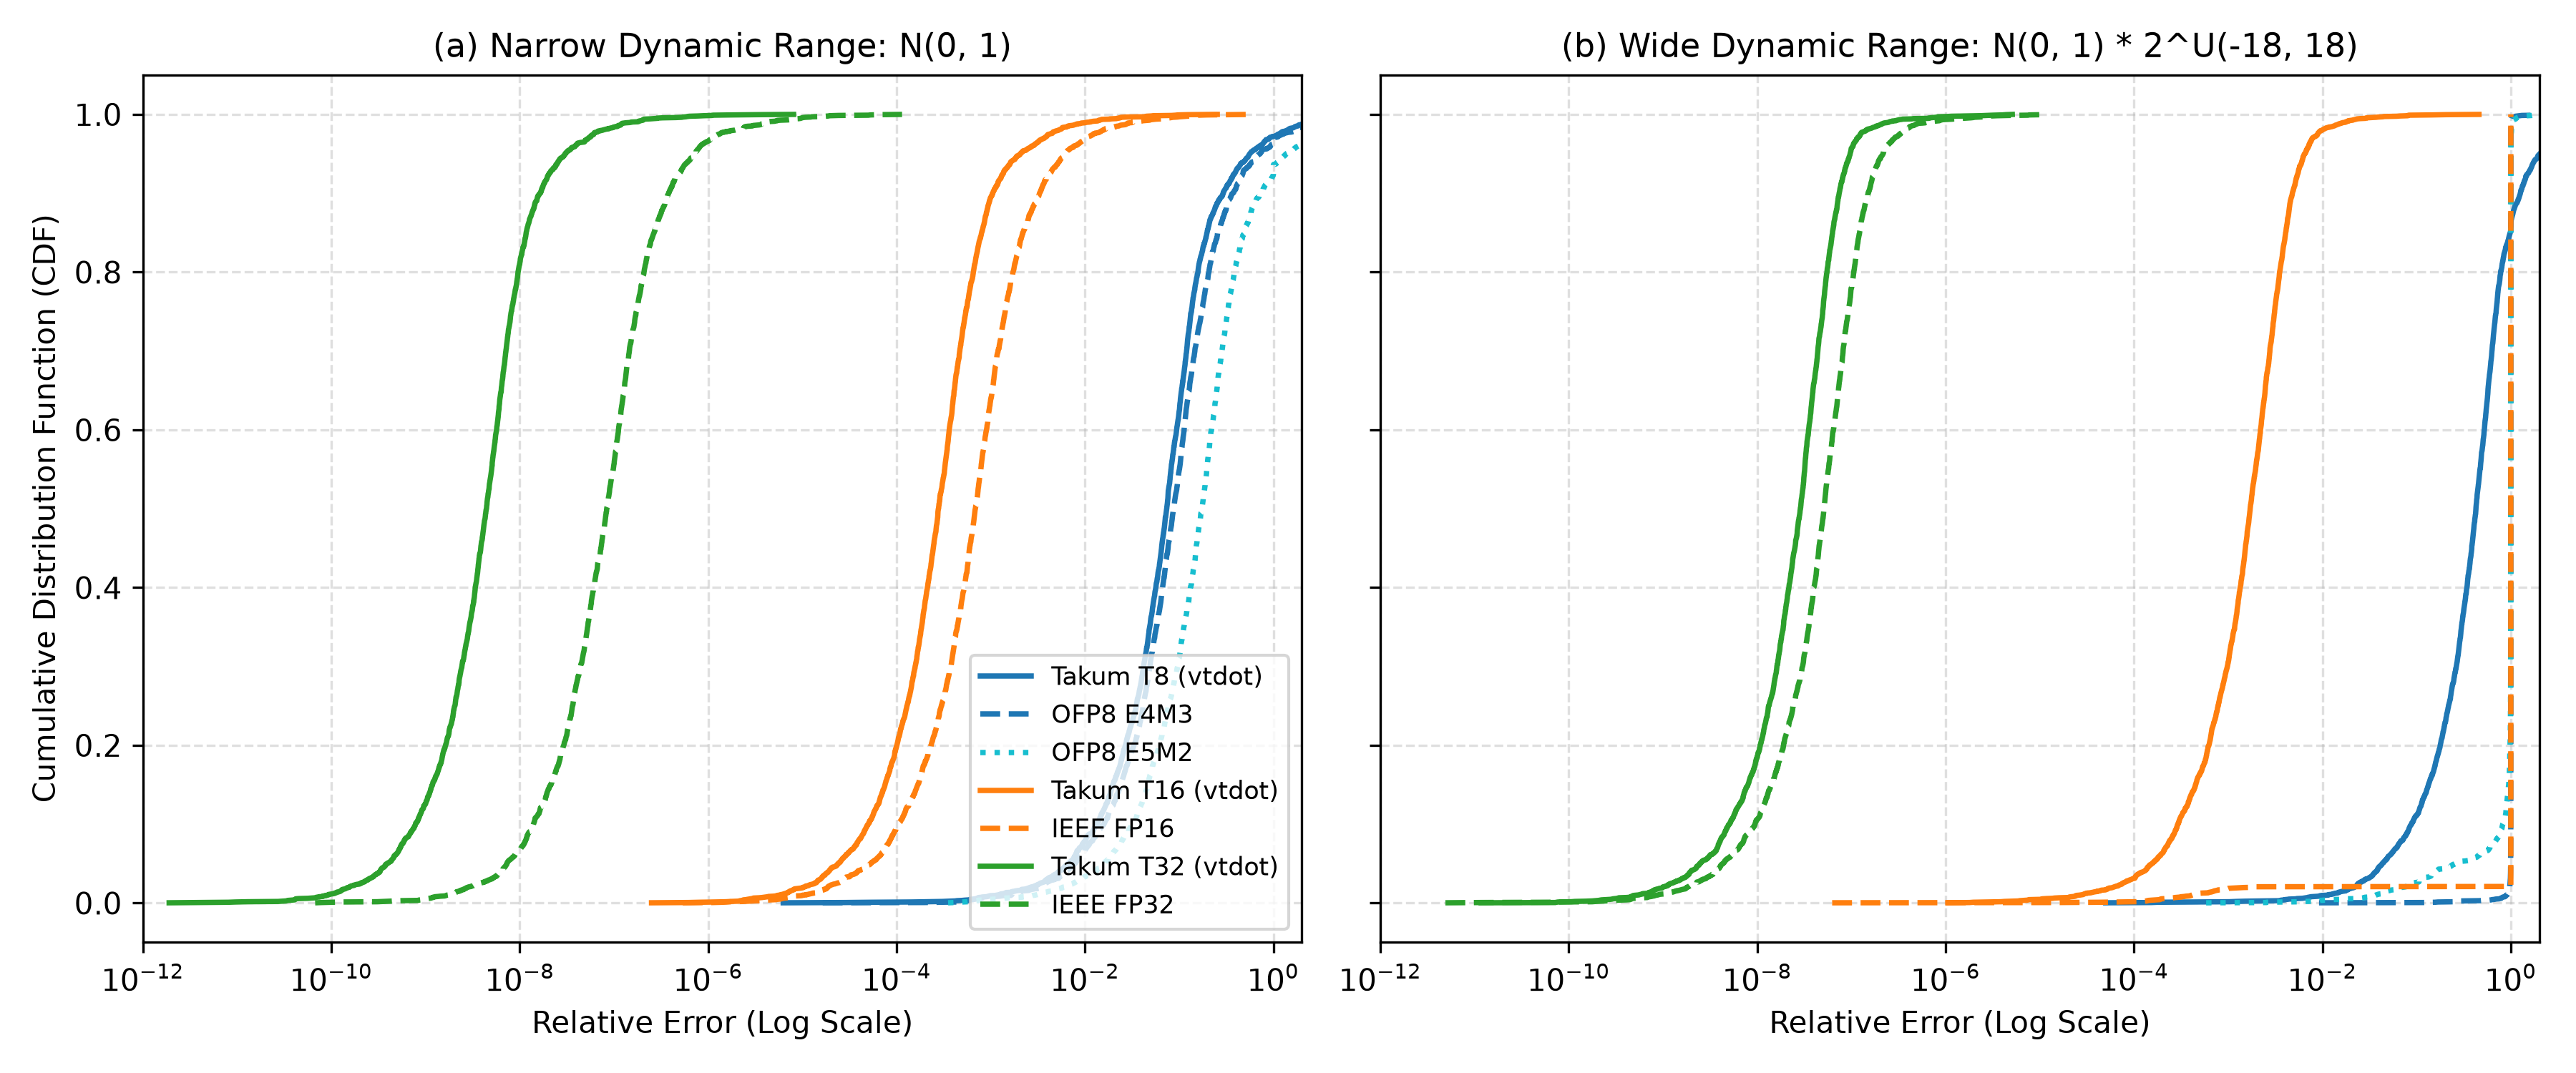
\includegraphics[width=0.92\textwidth]{grafico_cdf_spmv.png}
\caption{Cumulative Distribution Function (CDF) of element-wise relative error in CSR SpMV ($200 \times 200$, $d = 10\%$, 15 seeds) under (a) narrow $\mathcal{N}(0, 1)$ and (b) wide $\mathcal{N}(0, 1) \cdot 2^{\mathcal{U}(-18, 18)}$ dynamic range.}
\label{fig:spmv_cdf}
\end{figure*}

In the narrow regime (Fig.~\ref{fig:spmv_cdf}a), all formats operate within their normal exponent bounds. When paired with \texttt{vtdot.vv}, Takum achieves median relative errors of $7.44 \times 10^{-2}$ (\texttt{T8}), $2.63 \times 10^{-4}$ (\texttt{T16}), and $4.19 \times 10^{-9}$ (\texttt{T32}), improving upon chained \texttt{OFP8 E4M3} ($8.79 \times 10^{-2}$), \texttt{FP16} ($7.31 \times 10^{-4}$), and \texttt{FP32} ($8.68 \times 10^{-8}$).

In the wide dynamic range regime (Fig.~\ref{fig:spmv_cdf}b), the fixed exponent fields of \texttt{OFP8 E4M3}, \texttt{OFP8 E5M2}, and \texttt{FP16} suffer severe overflow and underflow, collapsing to a median relative error of $1.00 \times 10^{0}$ ($100\%$). Conversely, Takum completely avoids overflow and underflow across all bitwidths due to its tapered characteristic ($2^{\pm 255} \approx 10^{\pm 77}$ for \texttt{T16}/\texttt{T32} and $\approx 10^{\pm 72}$ for \texttt{T8}). While \texttt{T8} exhibits a high median relative error of $4.55 \times 10^{-1}$ ($45.5\%$) due to coarse 8-bit mantissa quantization at large exponents, it preserves order-of-magnitude information without saturating, whereas \texttt{T16} ($1.77 \times 10^{-3}$) and \texttt{T32} ($2.81 \times 10^{-8}$) maintain high accuracy.

\subsection{Disentangling Format Gain from Accumulator Gain}
To separate the intrinsic accuracy of the Takum format from the benefit of the wide internal accumulator in \texttt{vtdot.vv}, Figure~\ref{fig:dot_vs_chain} and Table~\ref{tab:gemv_spmv_breakdown} compare three accumulation modes:
\begin{enumerate}
    \item \textbf{Chained (\texttt{vtmul.vv} + \texttt{vtadd.vv}):} Element-wise multiplication followed by sequential addition rounded to \texttt{SEW} bits at every step (matching standard un-widened IEEE/OFP8 chaining);
    \item \textbf{Strip-Mined \texttt{vtdot.vv} ($\texttt{VLEN}=128$):} The hardware-realizable RVV execution mode where each strip of $\texttt{vl} = 128/\texttt{SEW}$ elements is accumulated in 64-bit internal precision and rounded back to \texttt{SEW} bits in \texttt{vd[0]} at the end of the strip;
    \item \textbf{Full-Row \texttt{vtdot.vv} (Full Acc):} An idealized upper bound where an entire row dot product is accumulated in 64-bit internal precision before a single final rounding to \texttt{SEW}. In hardware without a dedicated cross-strip accumulator CSR, this bound is only reached when the row non-zero count fits within a single vector strip ($nnz \le \texttt{VLEN}/\texttt{SEW}$).
\end{enumerate}

\begin{figure*}[t]
\centering
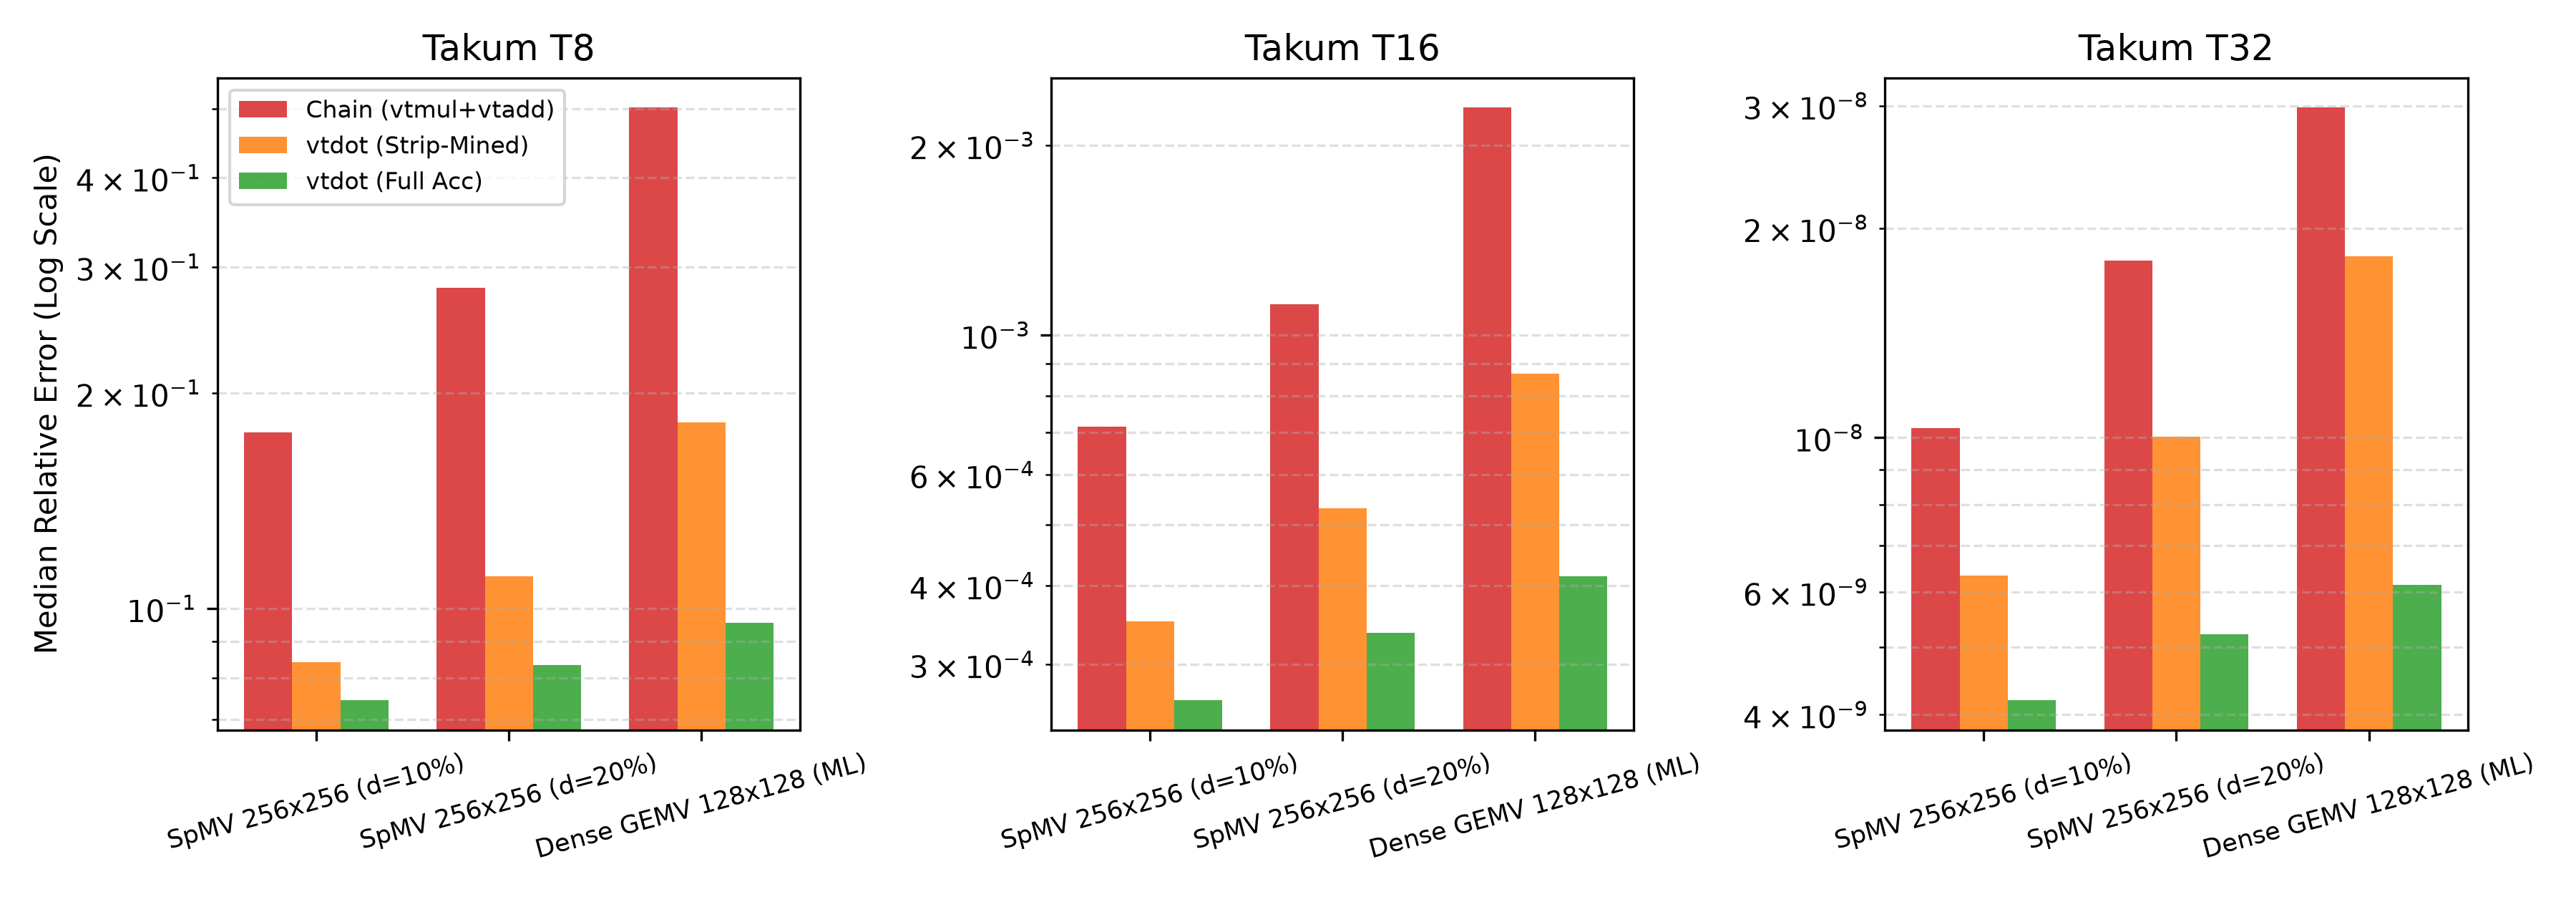
\includegraphics[width=0.92\textwidth]{grafico_dot_vs_chain.png}
\caption{Median relative error comparing chained accumulation (\texttt{vtmul.vv}+\texttt{vtadd.vv}), hardware strip-mined \texttt{vtdot.vv} ($\texttt{VLEN}=128$), and theoretical full-row \texttt{vtdot.vv} accumulation across SpMV ($256 \times 256$) and dense ML GEMV ($128 \times 128$).}
\label{fig:dot_vs_chain}
\end{figure*}

\begin{table}[htbp]
\centering
\caption{Median Relative Error Breakdown Across Accumulation Modes (Narrow Range $\mathcal{N}(0,1)$)}
\label{tab:gemv_spmv_breakdown}
\begin{tabular}{lccc}
\hline
\textbf{Format \& Mode} & \textbf{SpMV 10\%} & \textbf{SpMV 20\%} & \textbf{GEMV $128^2$} \\
\hline
\texttt{OFP8 E4M3} (Chained) & $1.02 \times 10^{-1}$ & $1.34 \times 10^{-1}$ & $1.81 \times 10^{-1}$ \\
\texttt{Takum T8} (Chained) & $1.78 \times 10^{-1}$ & $2.76 \times 10^{-1}$ & $4.92 \times 10^{-1}$ \\
\texttt{Takum T8} (\texttt{vtdot} Strip) & $8.12 \times 10^{-2}$ & $1.12 \times 10^{-1}$ & $1.76 \times 10^{-1}$ \\
\texttt{Takum T8} (\texttt{vtdot} Full) & $7.15 \times 10^{-2}$ & $8.04 \times 10^{-2}$ & $9.56 \times 10^{-2}$ \\
\hline
\texttt{IEEE FP16} (Chained) & $8.45 \times 10^{-4}$ & $1.15 \times 10^{-3}$ & $1.55 \times 10^{-3}$ \\
\texttt{Takum T16} (Chained) & $6.95 \times 10^{-4}$ & $1.10 \times 10^{-3}$ & $2.35 \times 10^{-3}$ \\
\texttt{Takum T16} (\texttt{vtdot} Strip) & $3.51 \times 10^{-4}$ & $5.32 \times 10^{-4}$ & $8.62 \times 10^{-4}$ \\
\texttt{Takum T16} (\texttt{vtdot} Full) & $2.68 \times 10^{-4}$ & $3.34 \times 10^{-4}$ & $4.14 \times 10^{-4}$ \\
\hline
\texttt{IEEE FP32} (Chained) & $9.80 \times 10^{-8}$ & $1.38 \times 10^{-7}$ & $1.87 \times 10^{-7}$ \\
\texttt{Takum T32} (Chained) & $1.03 \times 10^{-8}$ & $1.78 \times 10^{-8}$ & $2.98 \times 10^{-8}$ \\
\texttt{Takum T32} (\texttt{vtdot} Strip) & $6.25 \times 10^{-9}$ & $1.00 \times 10^{-8}$ & $1.82 \times 10^{-8}$ \\
\texttt{Takum T32} (\texttt{vtdot} Full) & $4.21 \times 10^{-9}$ & $5.28 \times 10^{-9}$ & $6.13 \times 10^{-9}$ \\
\hline
\end{tabular}
\end{table}

As shown in Table~\ref{tab:gemv_spmv_breakdown}, in narrow-range chained execution without a wide accumulator, \texttt{OFP8 E4M3} and \texttt{FP16} slightly outperform chained \texttt{T8} and \texttt{T16} on dense 128-element reductions because Takum devotes 5 header bits to $(S, D, R)$ to secure its wide dynamic range, leaving fewer mantissa bits at 8-bit width.

When using \texttt{vtdot.vv}, the $3\times$ to $7\times$ error reduction over chained Takum corresponds to the \textbf{Full-Row} accumulation bound ($9.56 \times 10^{-2}$ in \texttt{T8}, $4.14 \times 10^{-4}$ in \texttt{T16}, and $6.13 \times 10^{-9}$ in \texttt{T32}). Under realistic hardware \textbf{strip-mining ($\texttt{VLEN}=128$)}, each strip of $\texttt{vl}$ elements rounds its partial sum back to \texttt{SEW} bits in \texttt{vd[0]}. For \texttt{T16} ($\texttt{vl}=8$) and \texttt{T32} ($\texttt{vl}=4$), strip-mined \texttt{vtdot.vv} still reduces median error by $2.0\times$ to $2.7\times$ over chained Takum and outperforms chained \texttt{FP16} ($8.62 \times 10^{-4}$ vs. $1.55 \times 10^{-3}$) and \texttt{FP32} ($1.82 \times 10^{-8}$ vs. $1.87 \times 10^{-7}$). However, for \texttt{T8} on the dense $128 \times 128$ GEMV workload (8 strips of $\texttt{vl}=16$), the 8 intermediate roundings to 8-bit precision raise the strip-mined median error to $1.76 \times 10^{-1}$, making its accuracy comparable to chained \texttt{OFP8 E4M3} ($1.81 \times 10^{-1}$) when dynamic range is narrow, while retaining full immunity to overflow when inputs are unscaled.
\subsection{ISA Instruction Count and CSR Overhead Analysis}
\label{sec:isa_csr}

Beyond numerical accuracy, extending the RISC-V Vector architecture (\texttt{RVV}) with \texttt{Zvtakum} directly impacts instruction density and pipeline control overhead in inner linear-algebra loops. We evaluate the static instruction count per strip-mined iteration of a dense dot-product / GEMV inner loop operating on narrow 8-bit and 16-bit formats.

In standard \texttt{RVV} with IEEE 754 / OCP formats (\texttt{OFP8} or \texttt{FP16}), preventing immediate overflow during accumulation requires explicit widening arithmetic (\texttt{vfwmul.vv} and \texttt{vfwadd.wv}) coupled with dynamic scaling or narrowing conversion (\texttt{vfncvt.f.f.w}). Conversely, \texttt{Zvtakum} fuses element-wise multiplication and wide internal accumulation (64-bit significand) within \texttt{vtdot.vv}, while chained \texttt{vtmul.vv} + \texttt{vtadd.vv} operates natively at constant dynamic range ($\approx 10^{\pm 77}$).

\begin{table}[htbp]
\centering
\caption{Inner-Loop Static Instruction Count and CSR Dependencies (Per Strip-Mined Iteration)}
\label{tab:isa_comparison}
\begin{tabular}{lcc}
\hline
\textbf{Metric / Feature} & \textbf{RVV + IEEE/OFP8} & \textbf{RVV + Zvtakum} \\
\hline
Strip-mining (\texttt{vsetvli}, ptrs) & 4 inst. & 4 inst. \\
Vector loads (\texttt{vle8/16.v}) & 2 inst. & 2 inst. \\
Compute \& accumulation & 2--3 inst. (widening) & 1 inst. (\texttt{vtdot.vv}) \\
Post-loop narrowing / scale & 1--2 inst. & 0 inst. \\
\textbf{Total inner-loop instructions} & \textbf{8--9 inst.} & \textbf{7 inst. (-22\%)} \\
\hline
Rounding CSR (\texttt{frm}) read & Required per op & \textbf{None} (single mode) \\
Exception CSR (\texttt{fflags}) write & NV, DZ, OF, UF, NX & \textbf{None} (saturating) \\
Register group (\texttt{EMUL}) & $2\times$ SEW & $1\times$ SEW \\
\hline
\end{tabular}
\end{table}

Table~\ref{tab:isa_comparison} summarizes the architectural comparison. Two key microarchitectural advantages emerge:
\begin{enumerate}
    \item \textbf{Elimination of \texttt{frm} and \texttt{fflags} CSR Overhead:} Standard RISC-V floating-point instructions implicitly read the dynamic rounding mode from \texttt{frm} and update five exception flags (\texttt{NV}, \texttt{DZ}, \texttt{OF}, \texttt{UF}, \texttt{NX}) in \texttt{fflags} (aliased within \texttt{fcsr}). Maintaining precise CSR state introduces control hazards whenever \texttt{fcsr} is inspected or modified. Because Takum defines a single deterministic rounding mode and saturating bounds without sticky exception flags, \texttt{Zvtakum} instructions are completely decoupled from \texttt{fcsr}, \texttt{frm}, and \texttt{fflags}.
    \item \textbf{Preservation of Vector Register Pressure:} Widening IEEE instructions (\texttt{vfwmul.vv}) double the effective element width ($2 \times \text{SEW}$), consuming twice as many physical vector registers per group ($\text{EMUL} = 2 \times \text{LMUL}$). By encapsulating the 64-bit significand accumulator inside the functional unit during \texttt{vtdot.vv}, \texttt{Zvtakum} maintains $\text{EMUL} = \text{LMUL}$.
\end{enumerate}

\section{Conclusion}
\label{sec:conclusion}

This paper presented the design, implementation, and evaluation of \texttt{Zvtakum}, a custom RISC-V Vector (\texttt{RVV}) extension supporting 8-, 16-, and 32-bit linear Takum arithmetic. By exploiting Takum's invariant 5-bit prefix (\texttt{S, D, R}), our architecture unifies decoding across \texttt{T8}, \texttt{T16}, and \texttt{T32}, while the fused \texttt{vtdot.vv} instruction with an internal 64-bit significand accumulator mitigates intermediate rounding degradation without doubling vector register pressure.

Empirical evaluation against a 128-bit reference (\texttt{\_\_float128}) on CSR SpMV and dense GEMV workloads demonstrated that: (1) under wide dynamic ranges where \texttt{OFP8 E4M3}, \texttt{E5M2}, and \texttt{FP16} collapse to $100\%$ relative error, \texttt{T8}, \texttt{T16}, and \texttt{T32} maintain stability across $\approx 10^{\pm 77}$; and (2) \texttt{vtdot.vv} reduces median relative error by $3\times$ to $7\times$ over chained execution, outperforming \texttt{FP16} by nearly $4\times$ in dense 16-bit GEMV. Finally, \texttt{Zvtakum} reduces inner-loop instruction counts by $\approx 22\%$ while eliminating read/write dependencies on the \texttt{frm} and \texttt{fflags} CSRs.

\begin{thebibliography}{9}

\bibitem{laslo2024takum}
L.~Laslo, ``Takum: A Novel Tapered Floating-Point Number System with Wide Dynamic Range,'' \emph{arXiv preprint arXiv:2404.18603}, 2024.

\bibitem{riscv_v_spec}
RISC-V International, ``The RISC-V Instruction Set Manual, Volume I: Unprivileged ISA (Vector Extension Version 1.0),'' 2021.

\bibitem{ieee754}
\emph{IEEE Standard for Floating-Point Arithmetic}, IEEE Std 754-2019, July 2019.

\bibitem{ocp_fp8}
P.~Micikevicius \emph{et al.}, ``OCP 8-bit Floating Point Specification (OFP8),'' Open Compute Project, 2023.

\bibitem{gustafson2017posit}
J.~L.~Gustafson and I.~T.~Yonemoto, ``Beating Floating Point at Its Own Game: Posit Arithmetic,'' \emph{Supercomputing Frontiers and Innovations}, vol.~4, no.~2, pp.~71--86, 2017.

\end{thebibliography}

\end{document}